% subsubsection{Giao diện các bước tạo lộ trình}

% % \input{Images/8. Implement/Itinerary-UI/localhost-3000-planning-step1.png}
% % \input{Images/8. Implement/Itinerary-UI/localhost-3000-planning-step2.png}
% % \input{Images/8. Implement/Itinerary-UI/localhost-3000-planning-step3.png}
% % \input{Images/8. Implement/Itinerary-UI/localhost-3000-planning-step4.png}
% % \input{Images/8. Implement/Itinerary-UI/localhost-3000-planning-step5.png}
% % \input{Images/8. Implement/Itinerary-UI/localhost-3000-planning-summary.png}

\subsubsection{Giao diện các bước tạo lộ trình}

Quá trình tạo lịch trình du lịch thông minh được chia thành 6 bước tuần tự. Giao diện được thiết kế trực quan giúp thu thập đầy đủ dữ liệu đầu vào.

% --- BƯỚC 1 ---
\begin{figure}[H]
    \centering
    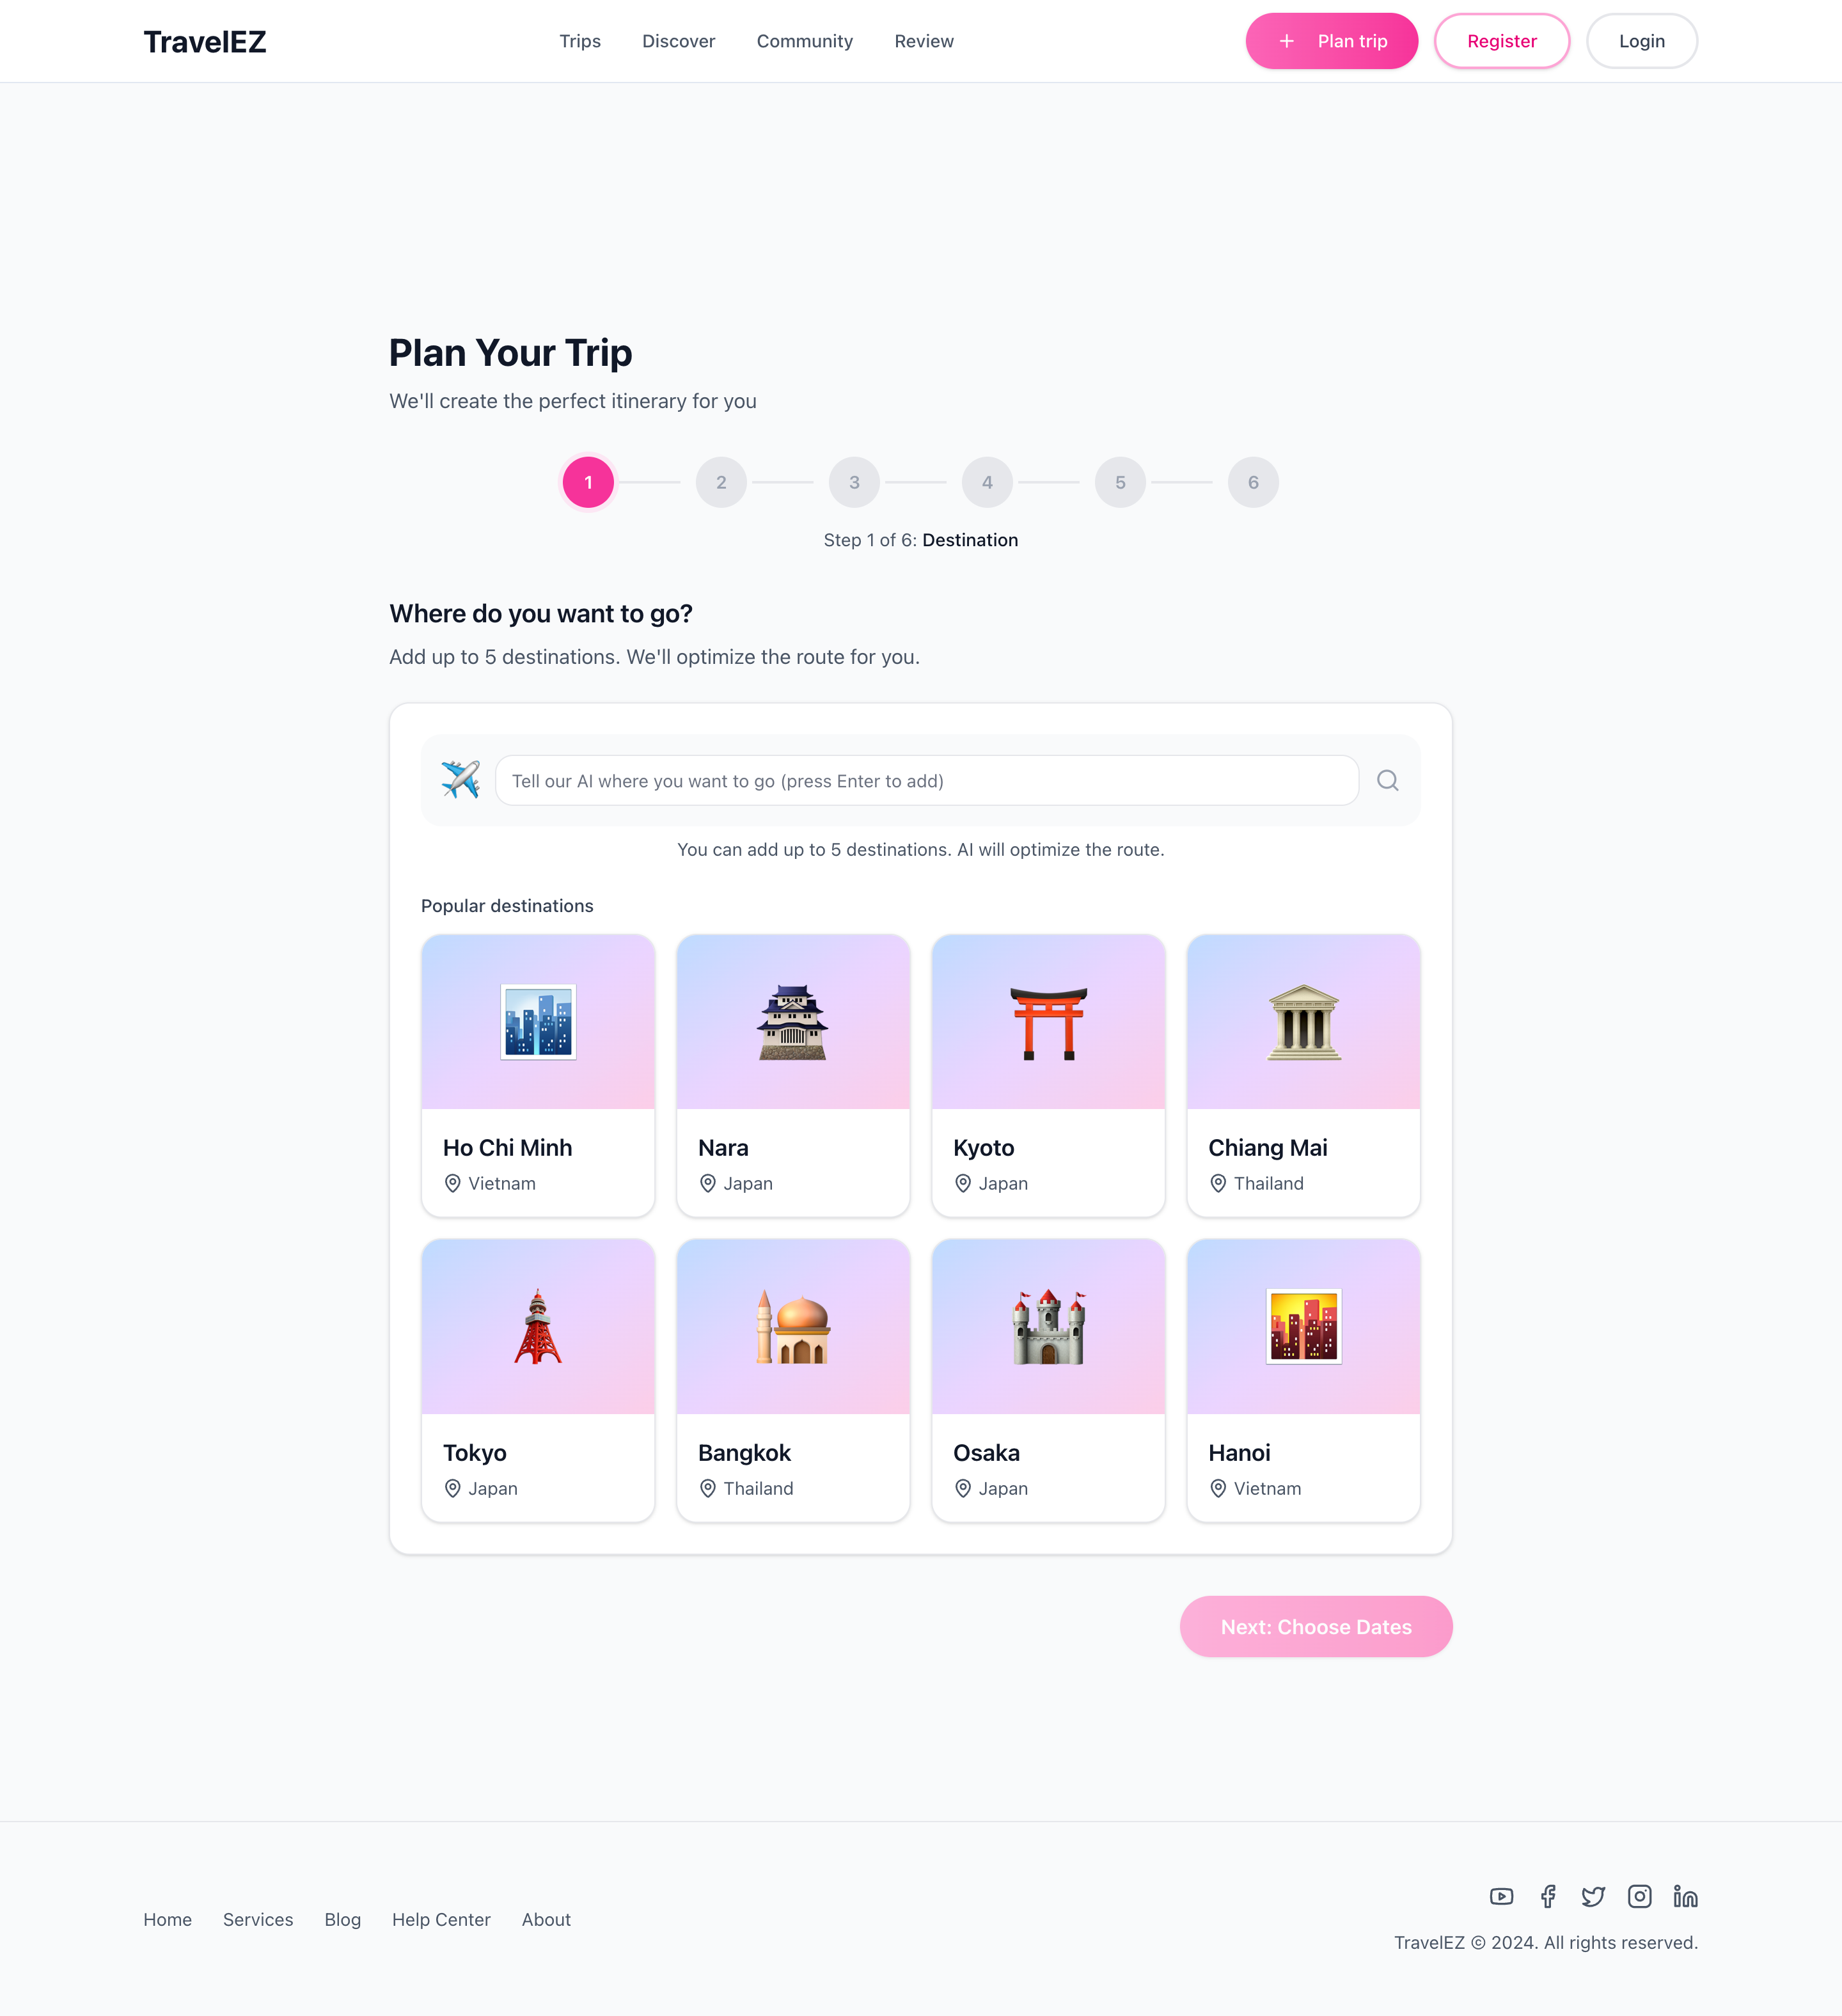
\includegraphics[width=1.0\linewidth]{Images/8. Implement/Itinerary-UI/localhost-3000-planning-step1.png}
    \caption{Giao diện Bước 1: Lựa chọn điểm đến (Destination)}
    \label{fig:step1}
    
    \vspace{0.5cm}
    
    \raggedright
    \textbf{Bước 1 - Lựa chọn điểm đến:} Tại màn hình khởi đầu, người dùng nhập tên thành phố hoặc địa danh muốn đến vào thanh tìm kiếm. Hệ thống hỗ trợ cơ chế "Multi-destination" (đa điểm đến), AI sẽ tính toán thứ tự di chuyển tối ưu.
\end{figure}

% --- BƯỚC 2 ---
\begin{figure}[H]
    \centering
    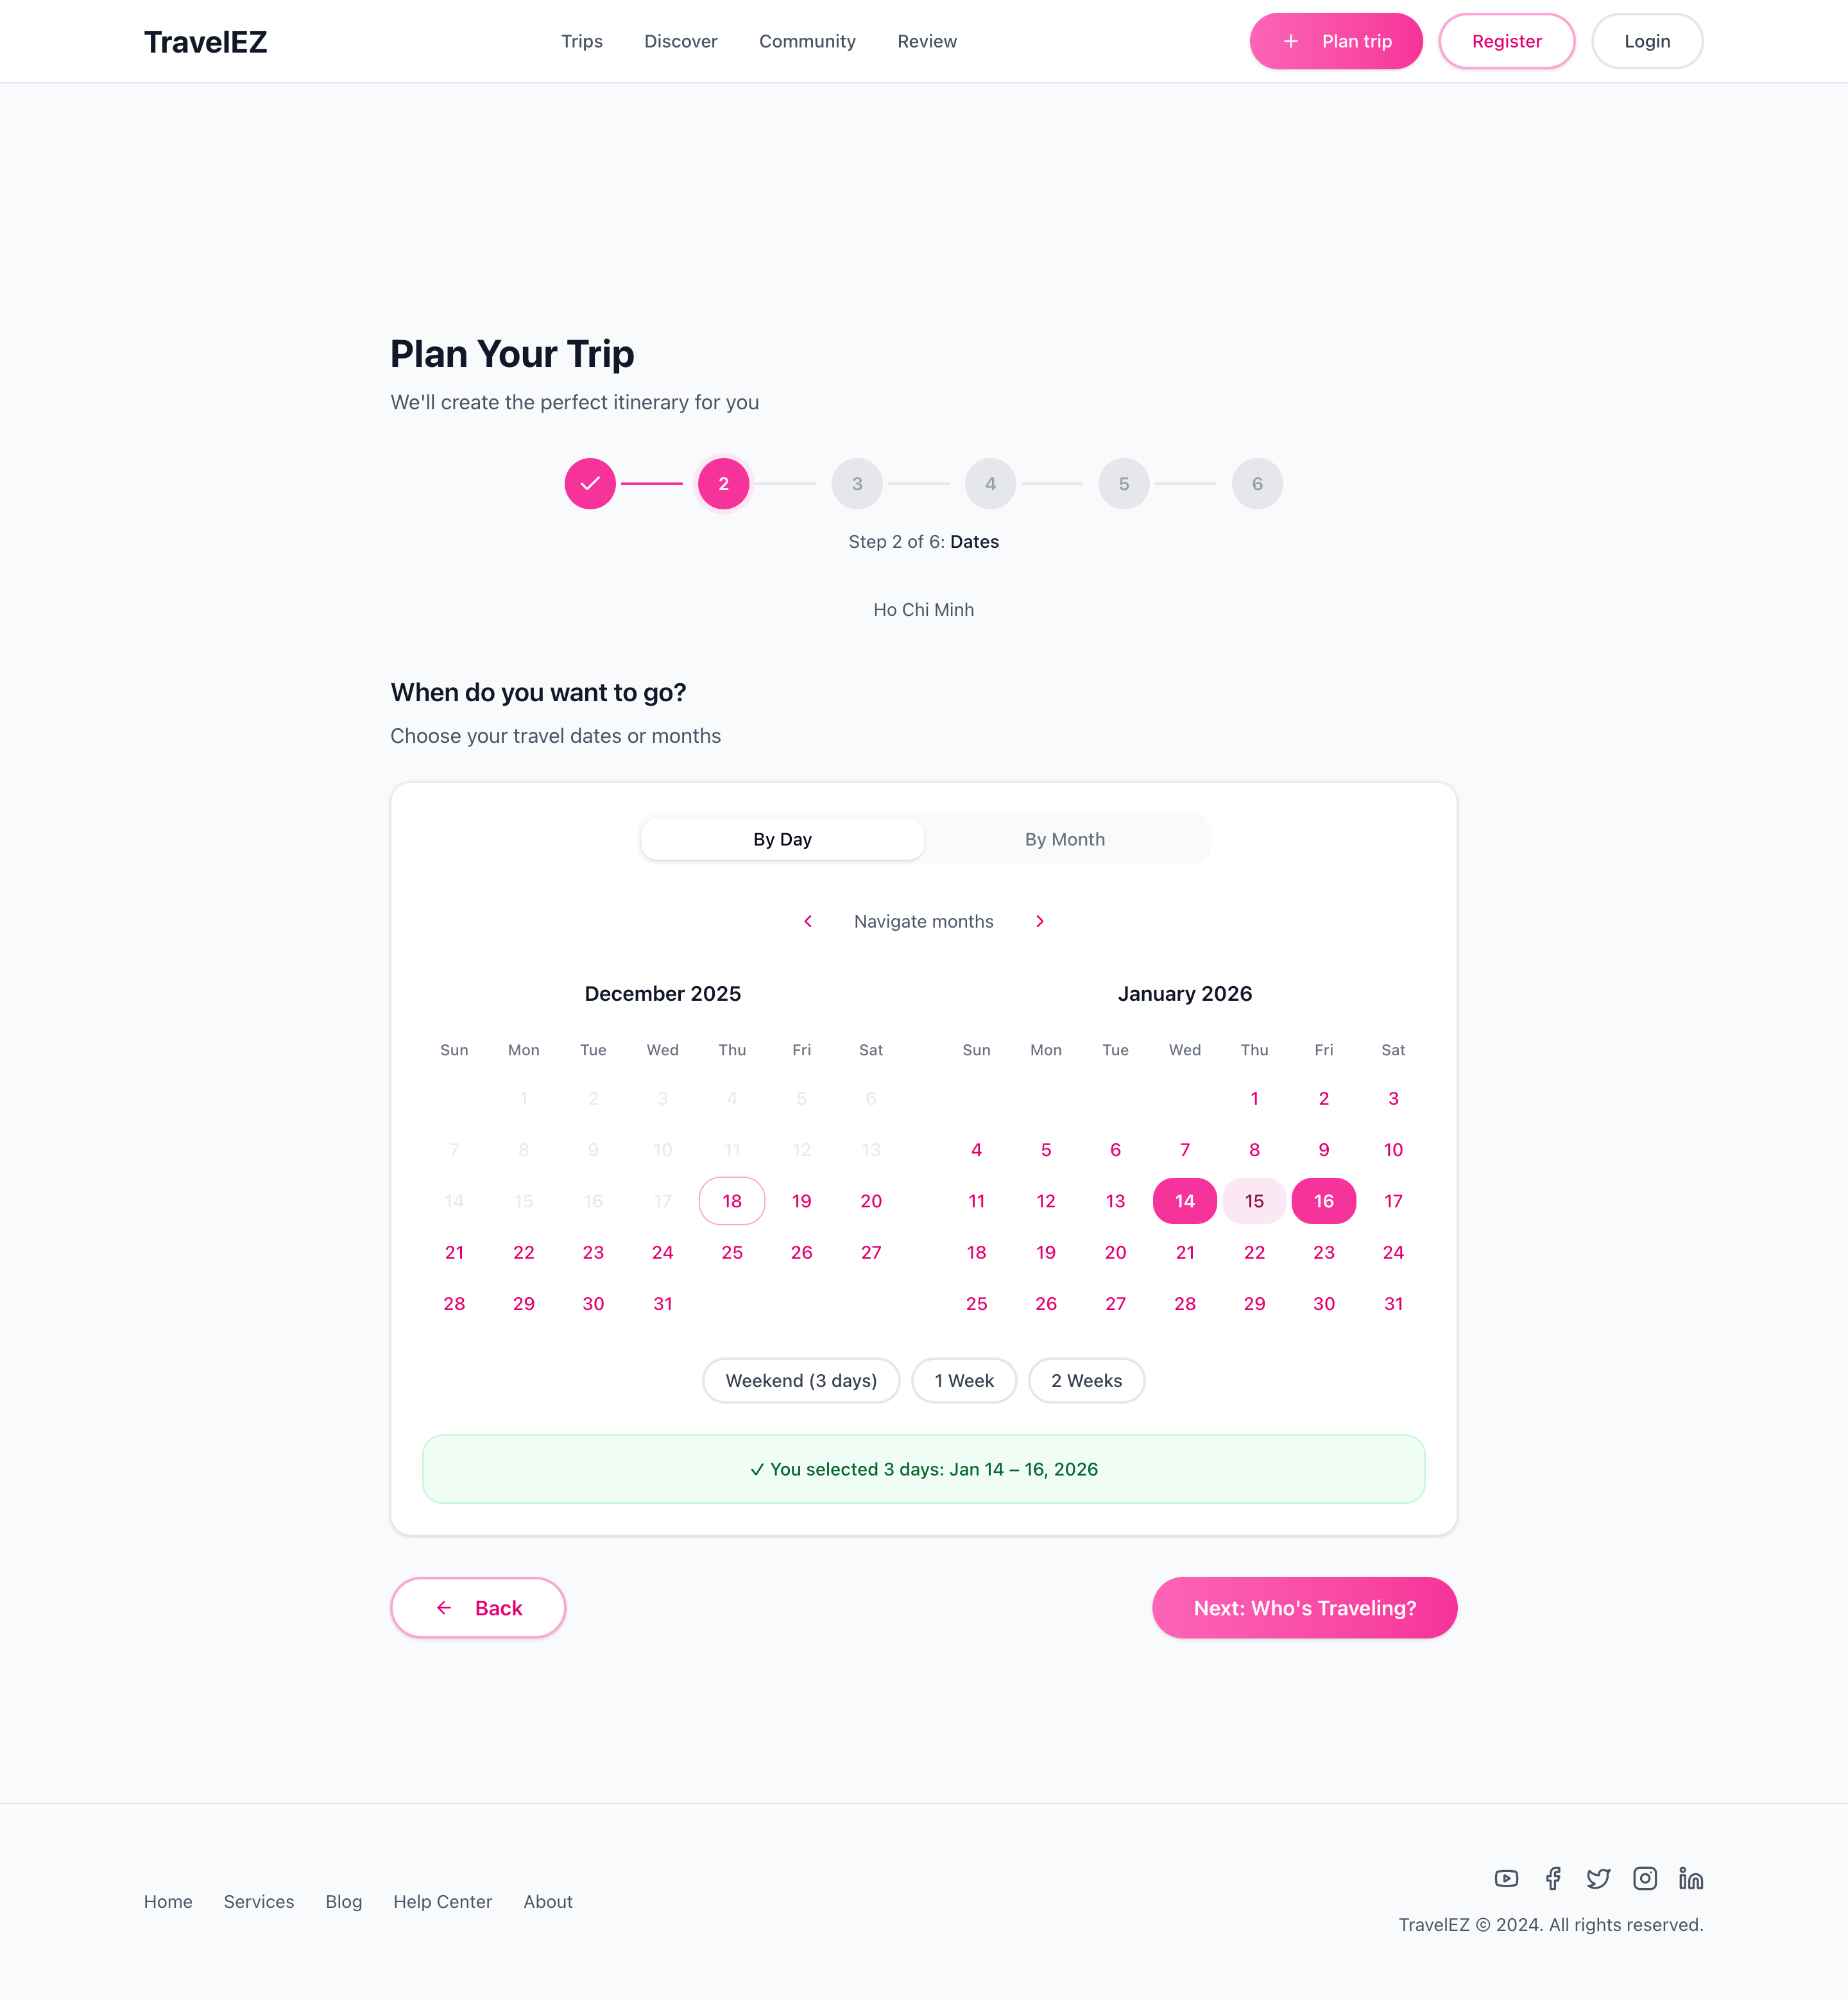
\includegraphics[width=1.0\linewidth]{Images/8. Implement/Itinerary-UI/localhost-3000-planning-step2.png}
    \caption{Giao diện Bước 2: Chọn thời gian khởi hành (Dates)}
    \label{fig:step2}
    
    \vspace{0.5cm}
    \raggedright
    \textbf{Bước 2 - Xác định thời gian:} Người dùng xác định khoảng thời gian thông qua giao diện lịch (Calendar View). Hệ thống hỗ trợ chọn ngày cụ thể hoặc theo tháng dự kiến để AI lọc các sự kiện phù hợp.
\end{figure}

% --- BƯỚC 3 ---
\begin{figure}[H]
    \centering
    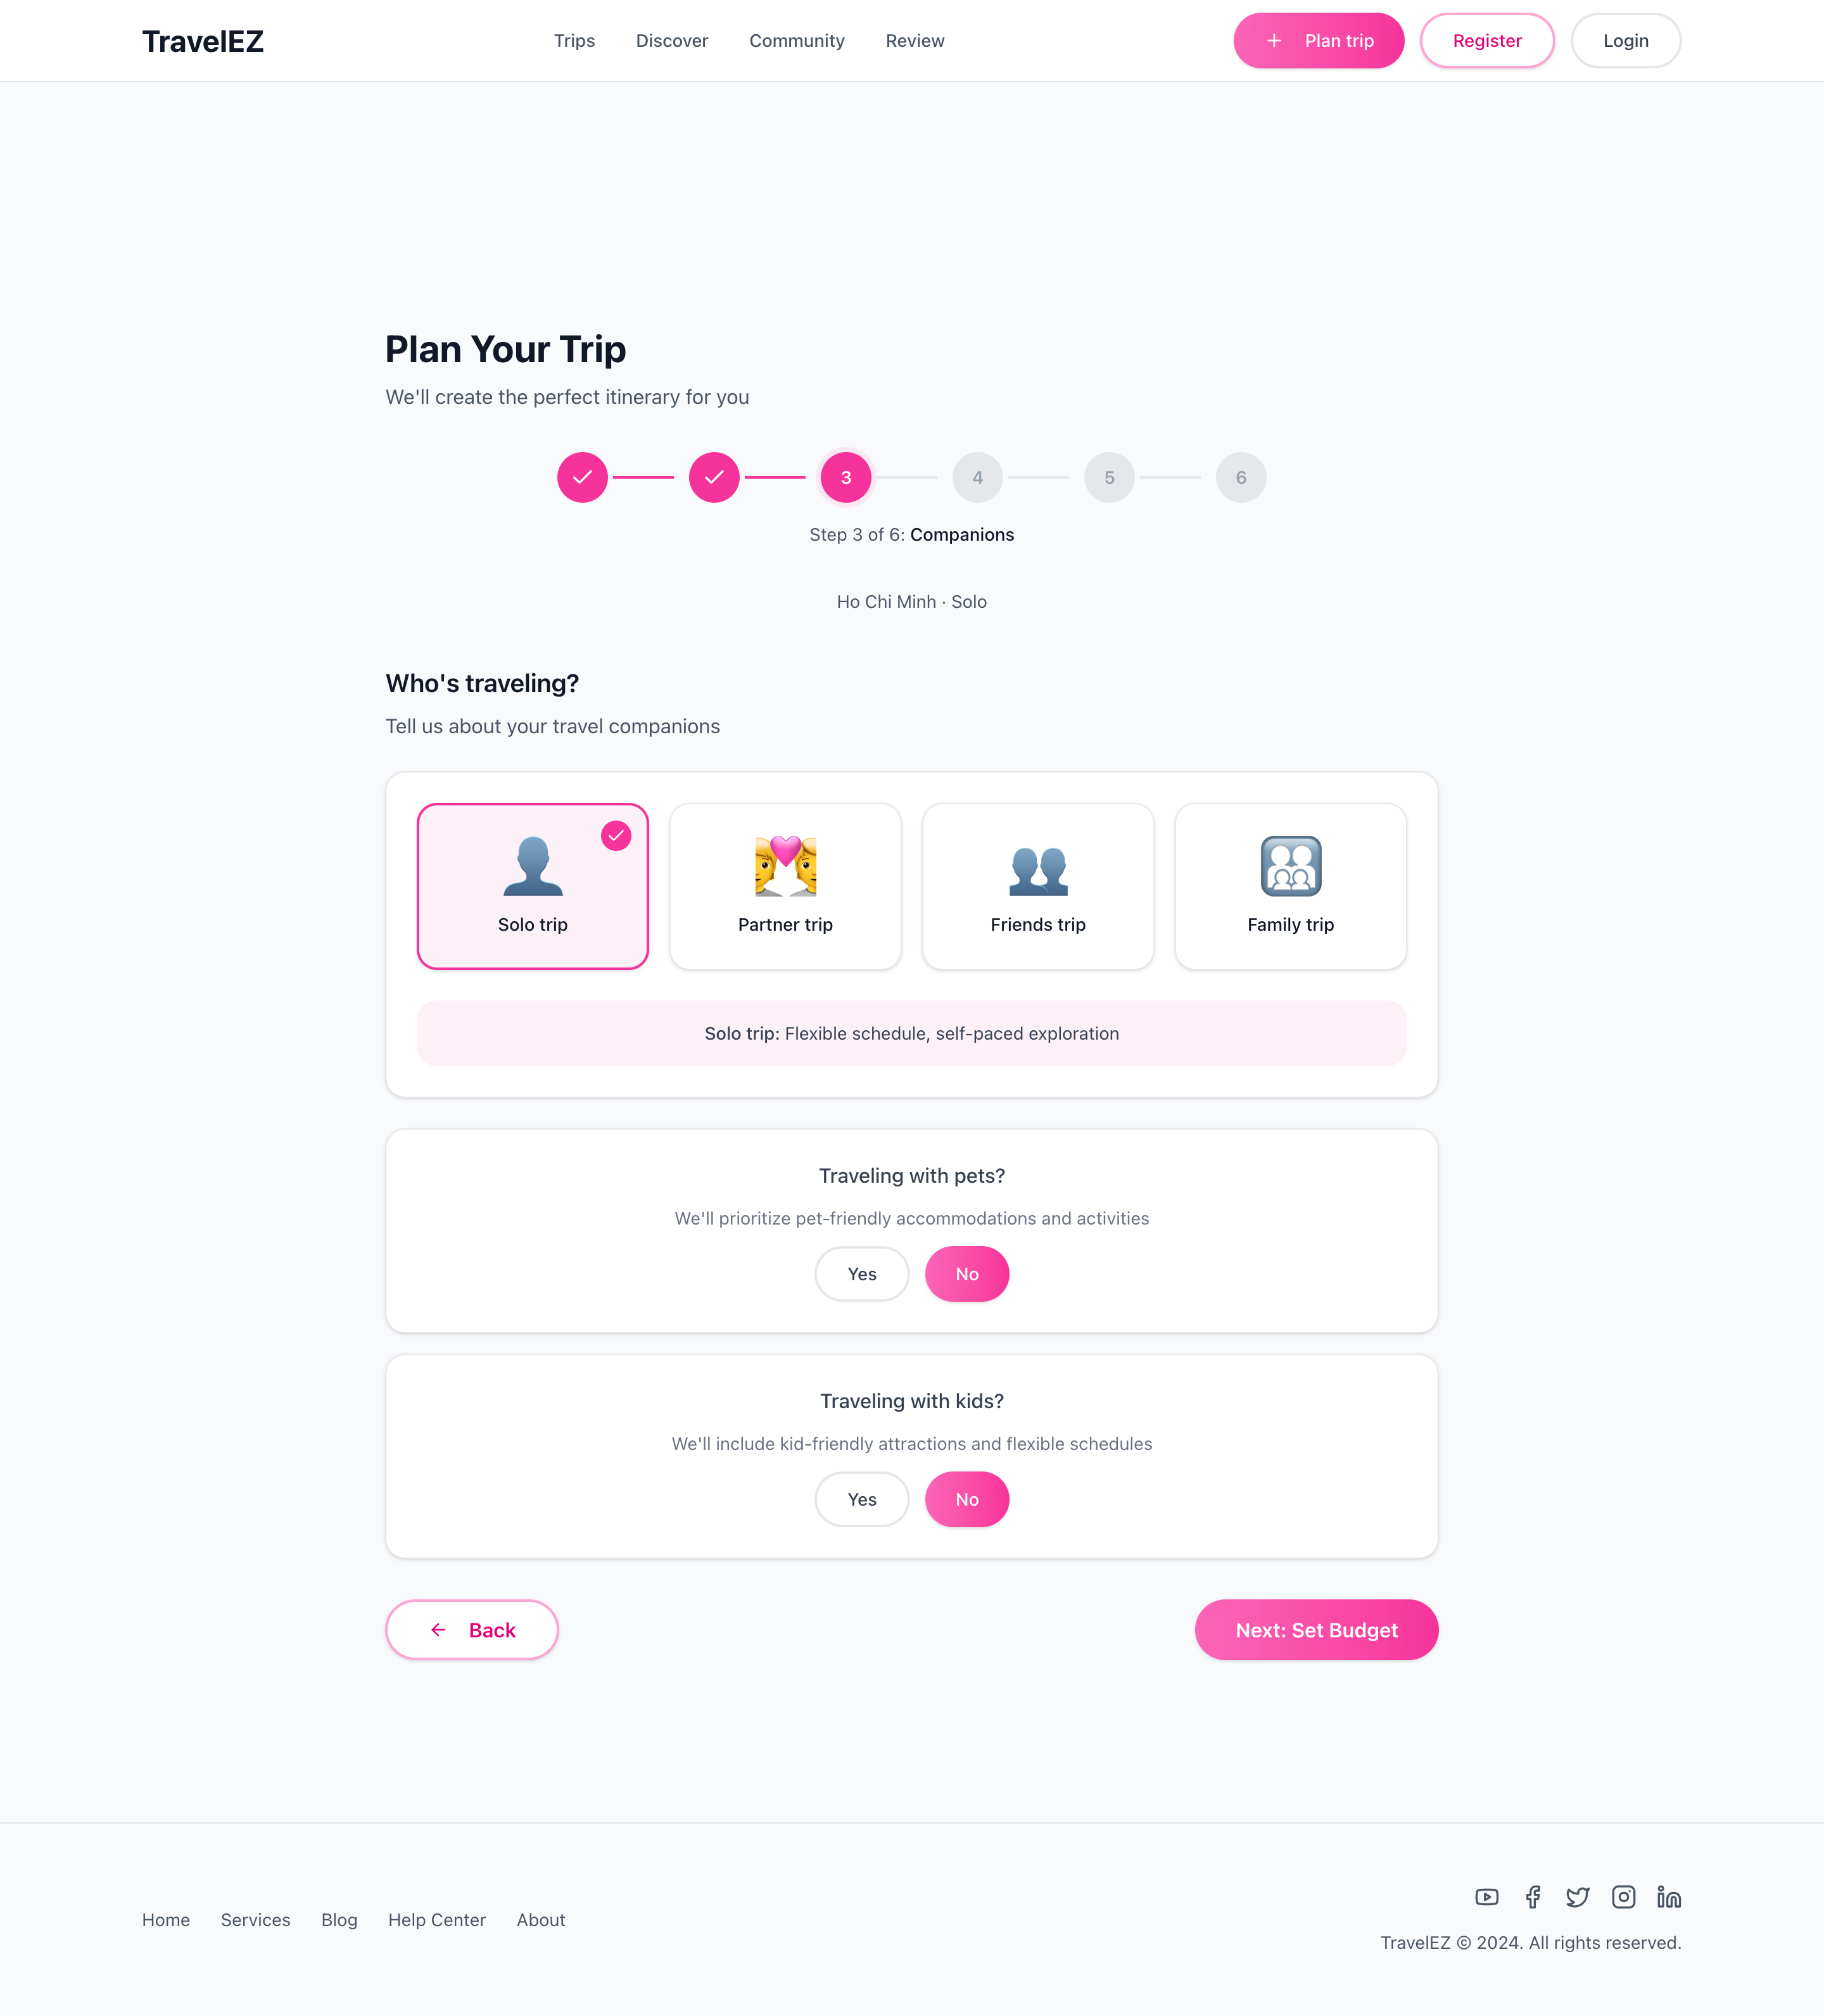
\includegraphics[width=1.0\linewidth]{Images/8. Implement/Itinerary-UI/localhost-3000-planning-step3.png}
    \caption{Giao diện Bước 3: Chọn người đồng hành (Companions)}
    \label{fig:step3}
    
    \vspace{0.5cm}
    \raggedright
    \textbf{Bước 3 - Thông tin hành khách:} Thu thập bối cảnh chuyến đi (Solo, Gia đình, Nhóm bạn...). Tùy chọn "Mang thú cưng" hay "Có trẻ nhỏ" là bộ lọc quan trọng để loại bỏ các địa điểm không phù hợp.
\end{figure}

% --- BƯỚC 4 ---
\begin{figure}[H]
    \centering
    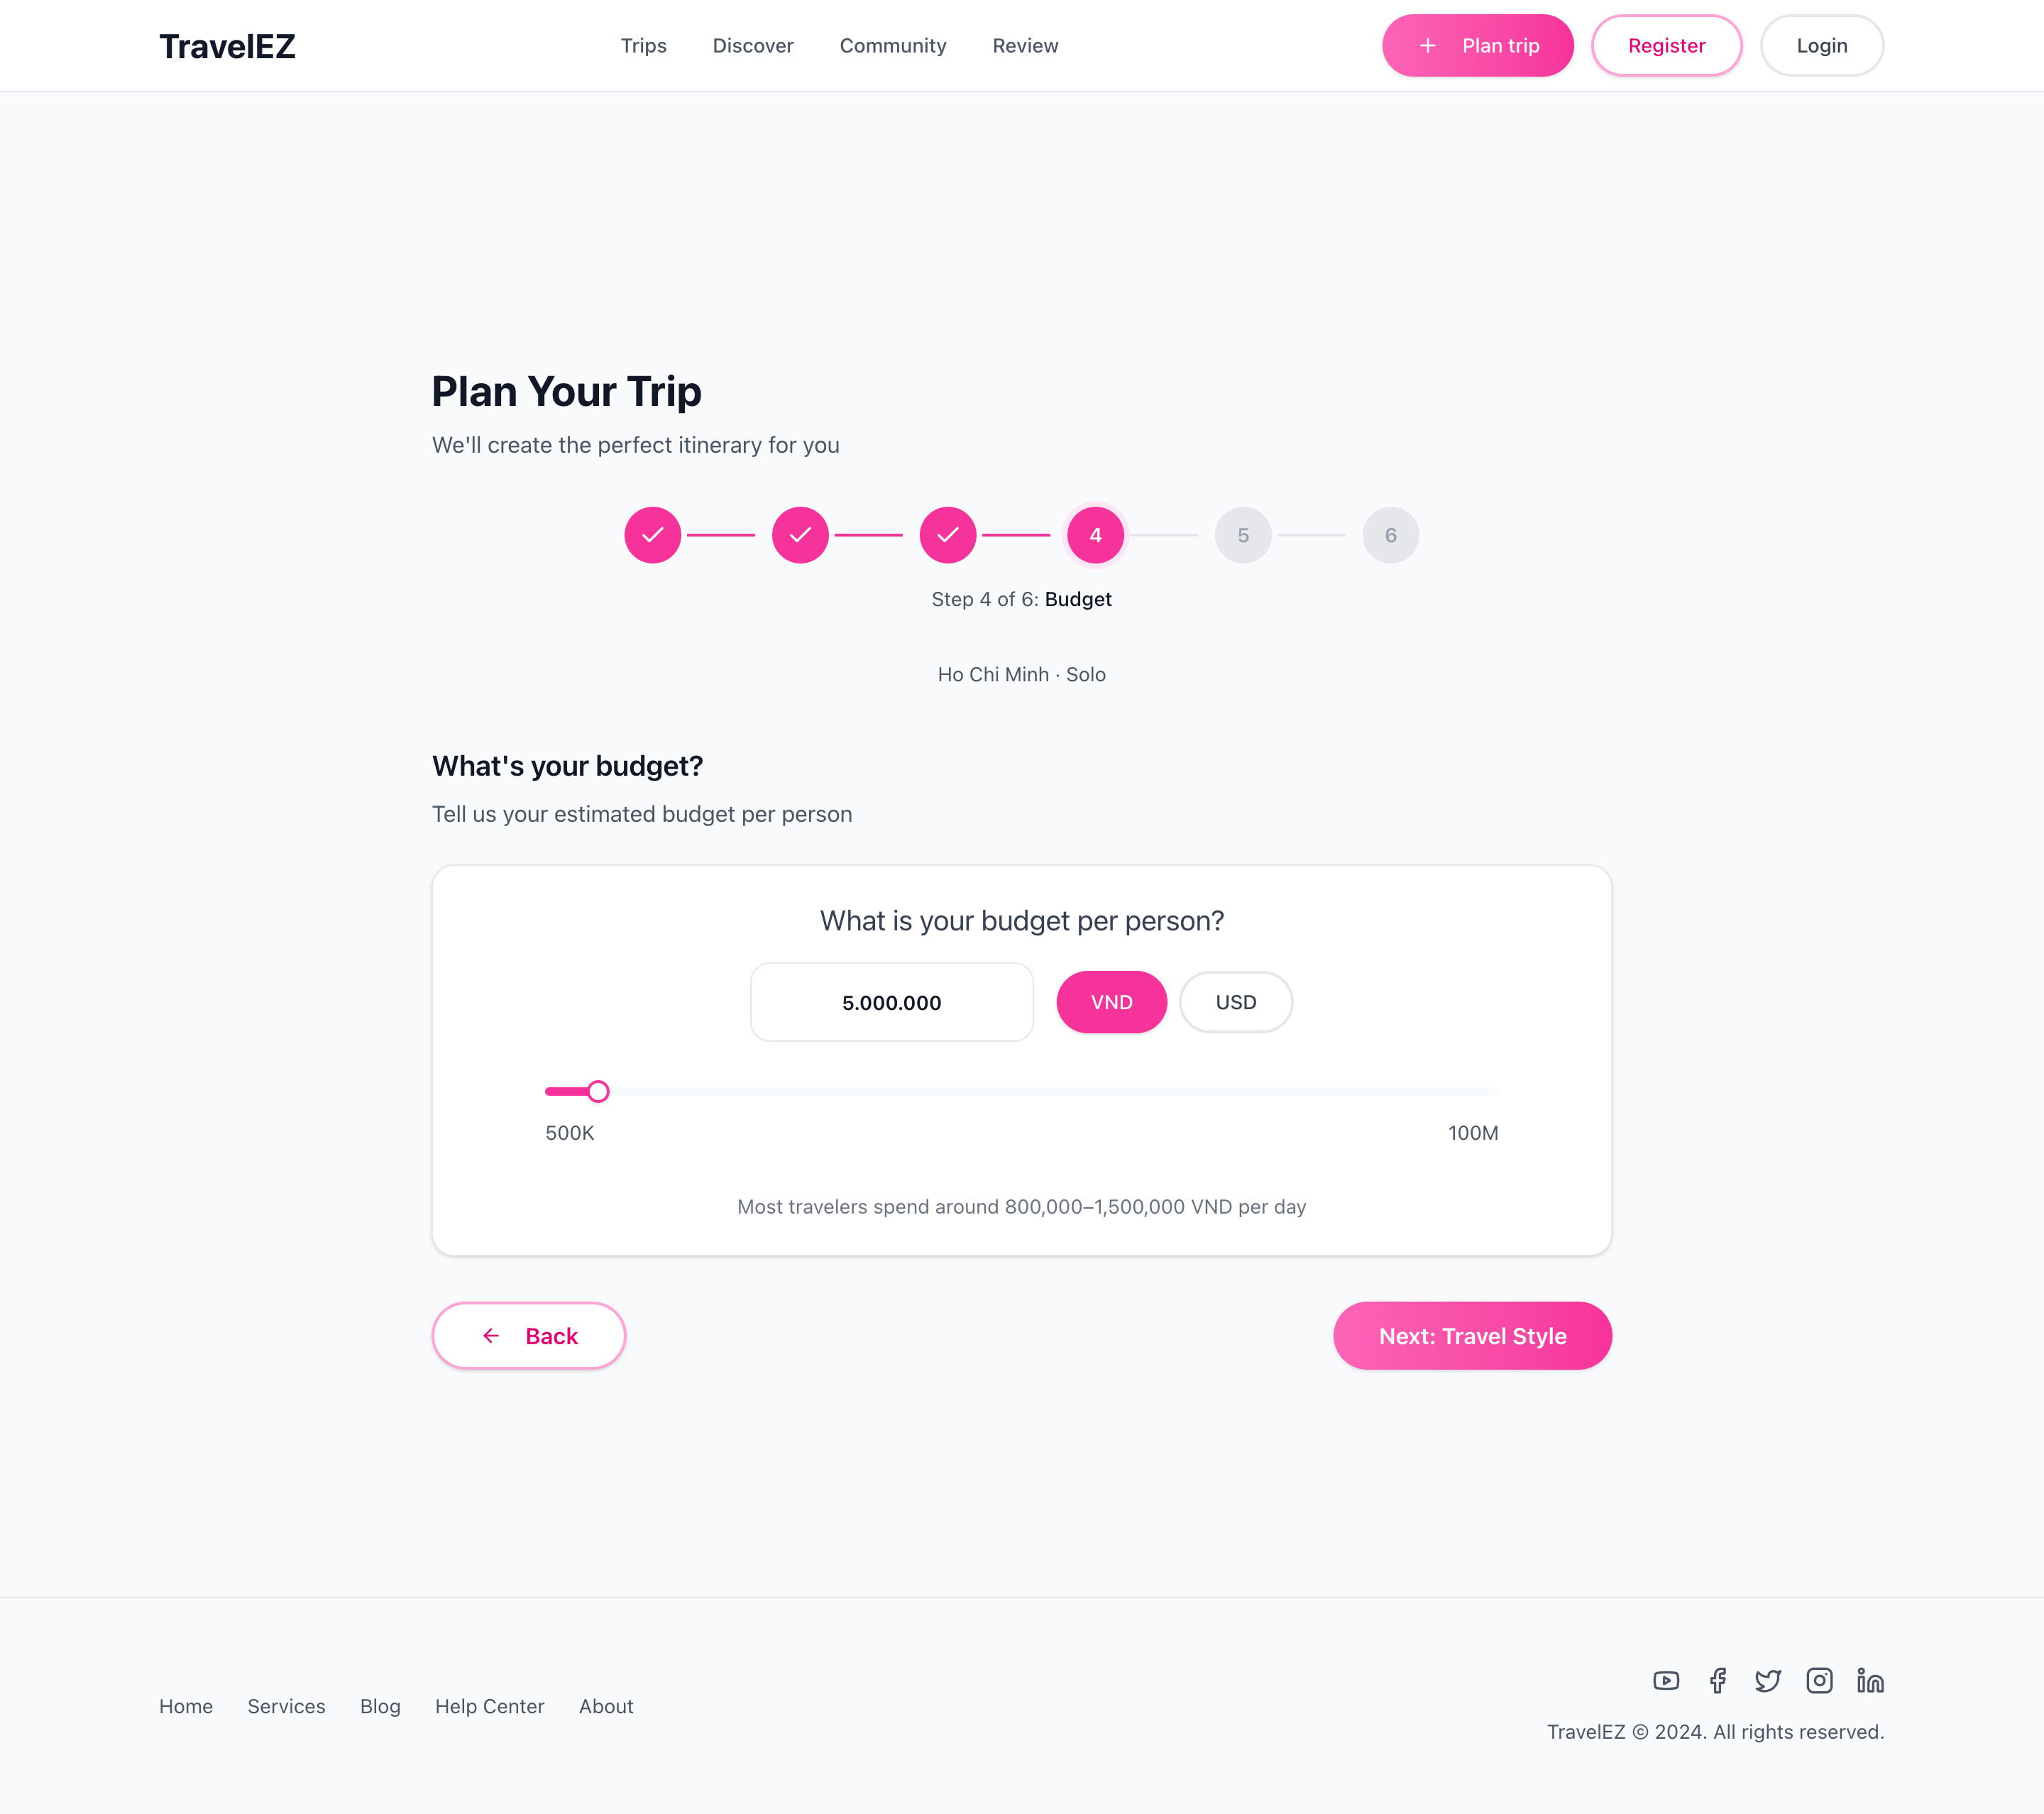
\includegraphics[width=1.0\linewidth]{Images/8. Implement/Itinerary-UI/localhost-3000-planning-step4.png}
    \caption{Giao diện Bước 4: Thiết lập ngân sách (Budget)}
    \label{fig:step4}
    
    \vspace{0.5cm}
    \raggedright
    \textbf{Bước 4 - Dự toán ngân sách:} Thanh trượt (Slider) giúp thiết lập giới hạn chi tiêu (VND/USD). Hệ thống dựa vào đây để gợi ý dịch vụ lưu trú, ăn uống vừa túi tiền.
\end{figure}

% --- BƯỚC 5 ---
\begin{figure}[H]
    \centering
    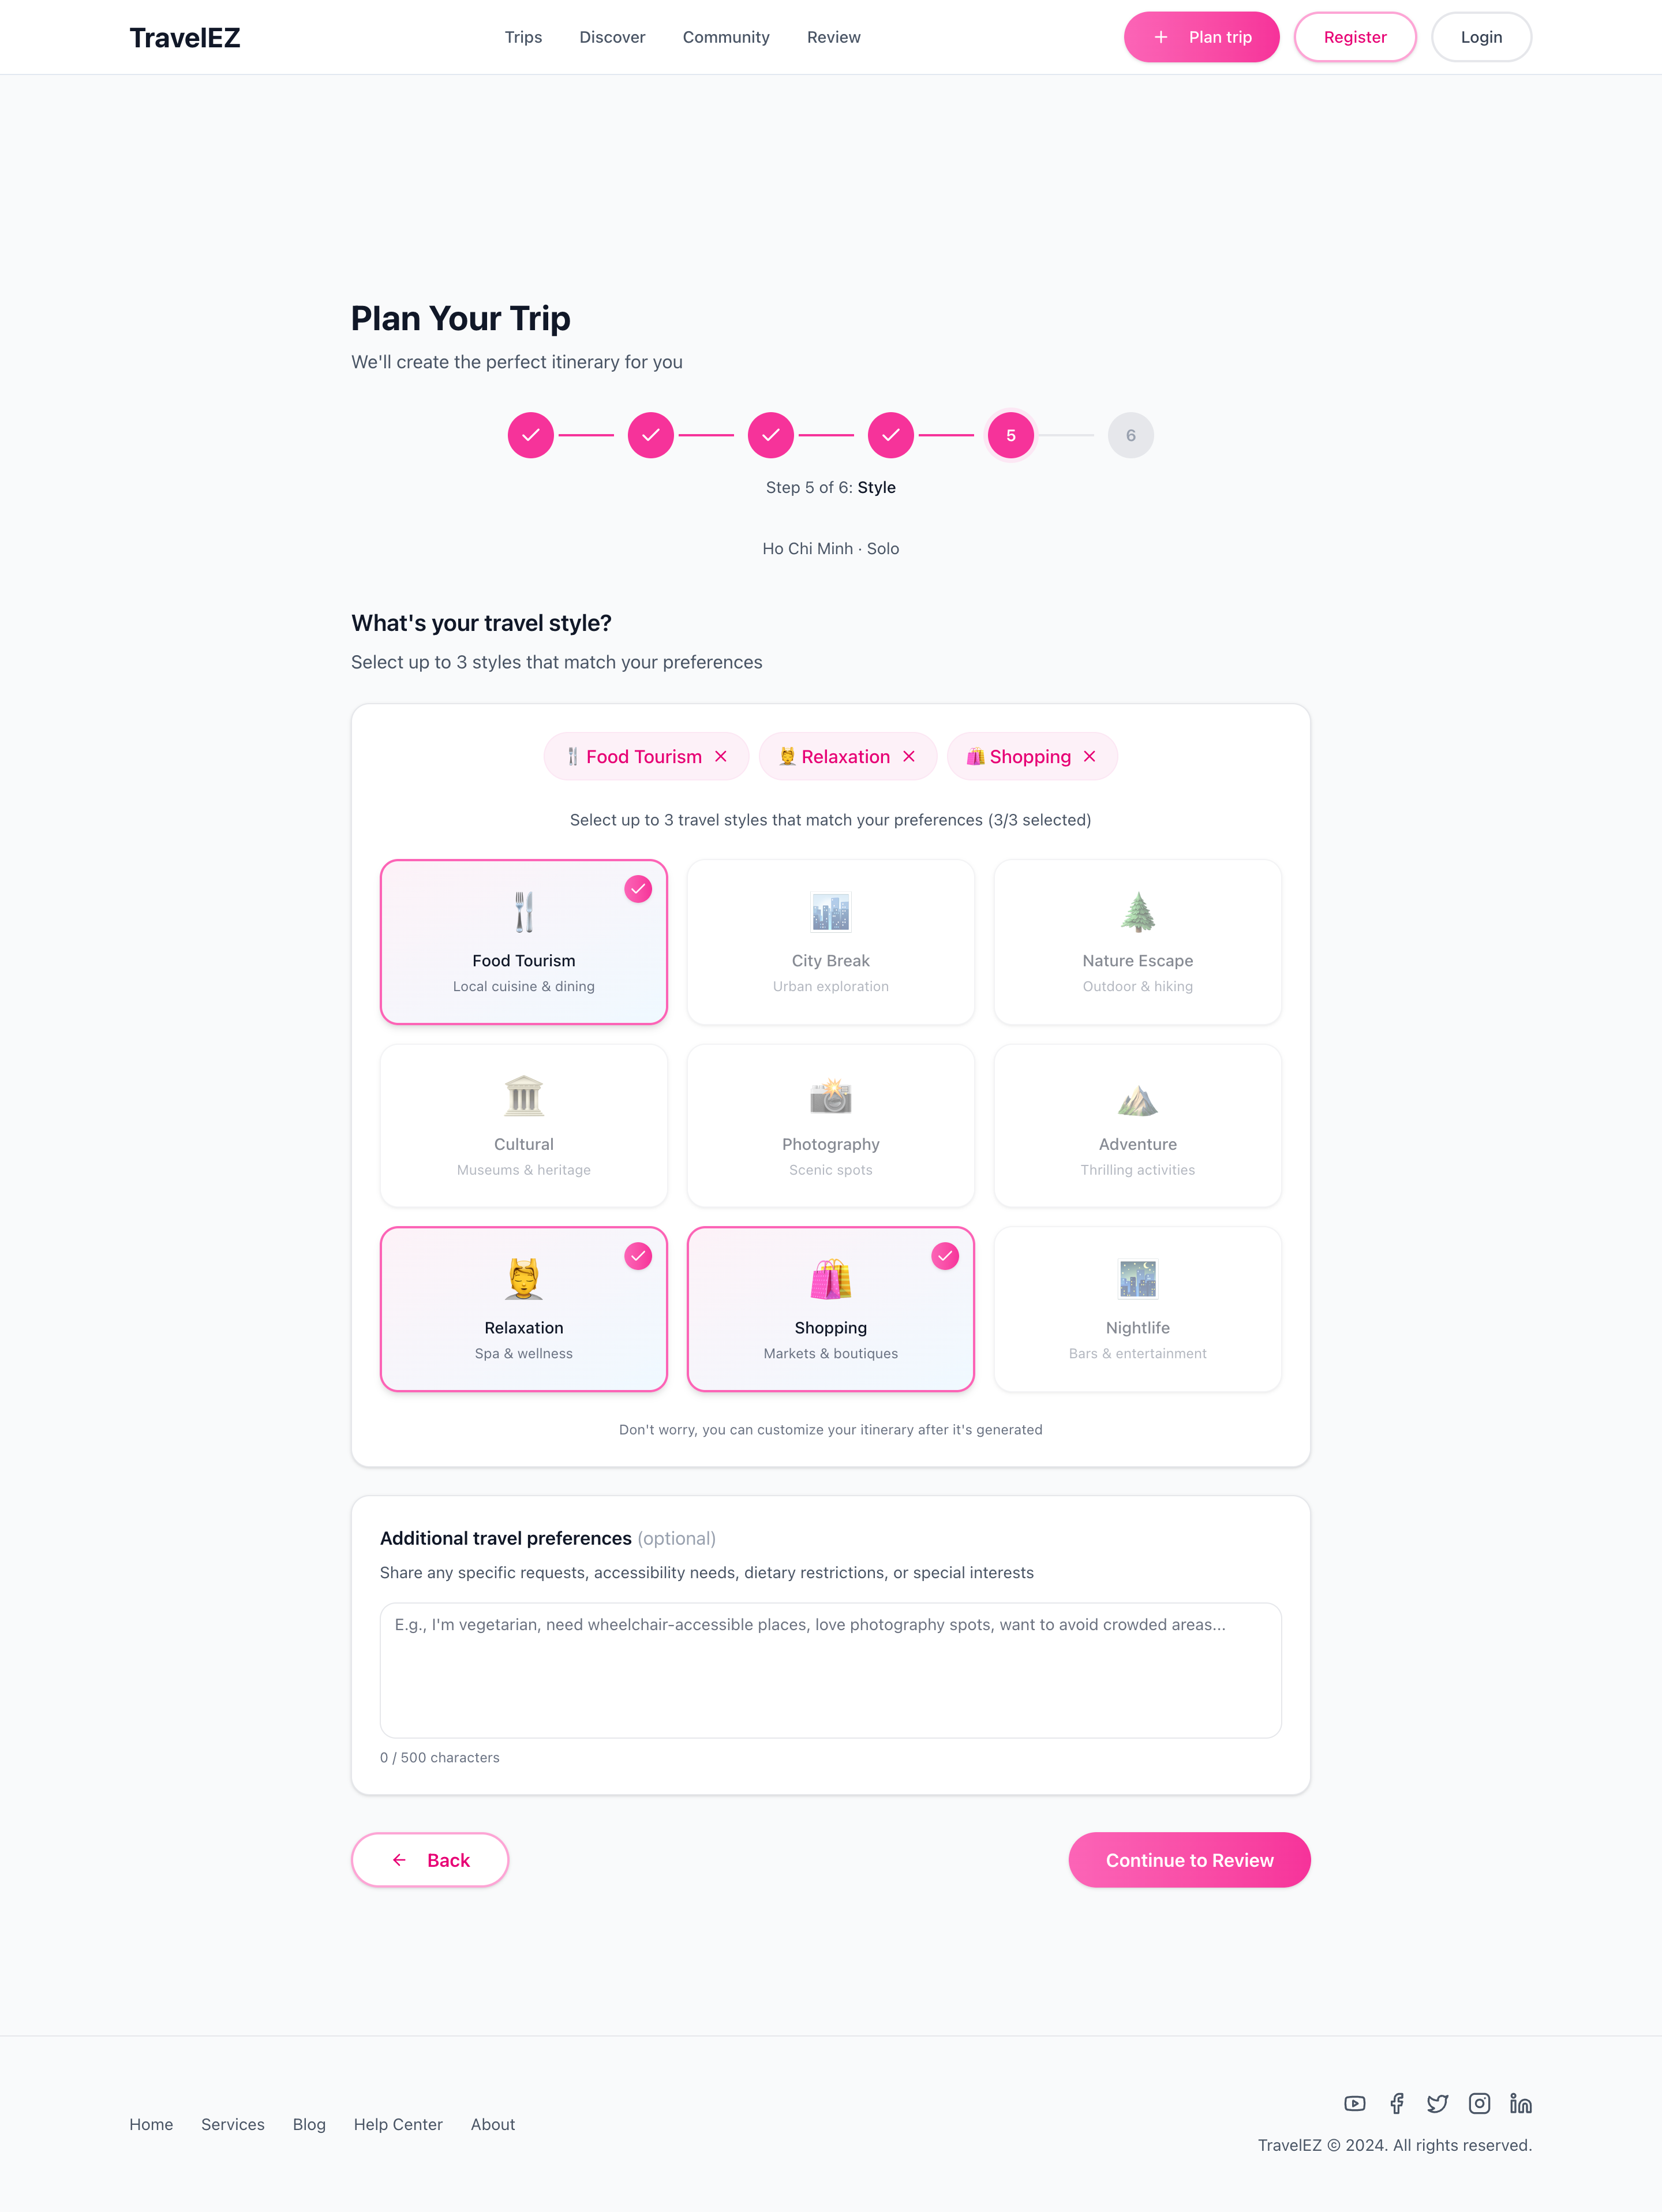
\includegraphics[width=1.0\linewidth]{Images/8. Implement/Itinerary-UI/localhost-3000-planning-step5.png}
    \caption{Giao diện Bước 5: Chọn phong cách du lịch (Travel Style)}
    \label{fig:step5}
    
    \vspace{0.5cm}
    \raggedright
    \textbf{Bước 5 - Định hình phong cách:} Người dùng chọn thẻ sở thích (Ẩm thực, Nghỉ dưỡng...) hoặc nhập yêu cầu đặc biệt bằng ngôn ngữ tự nhiên vào ô "Additional preferences" để NLP xử lý.
\end{figure}

% --- SUMMARY ---
\begin{figure}[H]
    \centering
    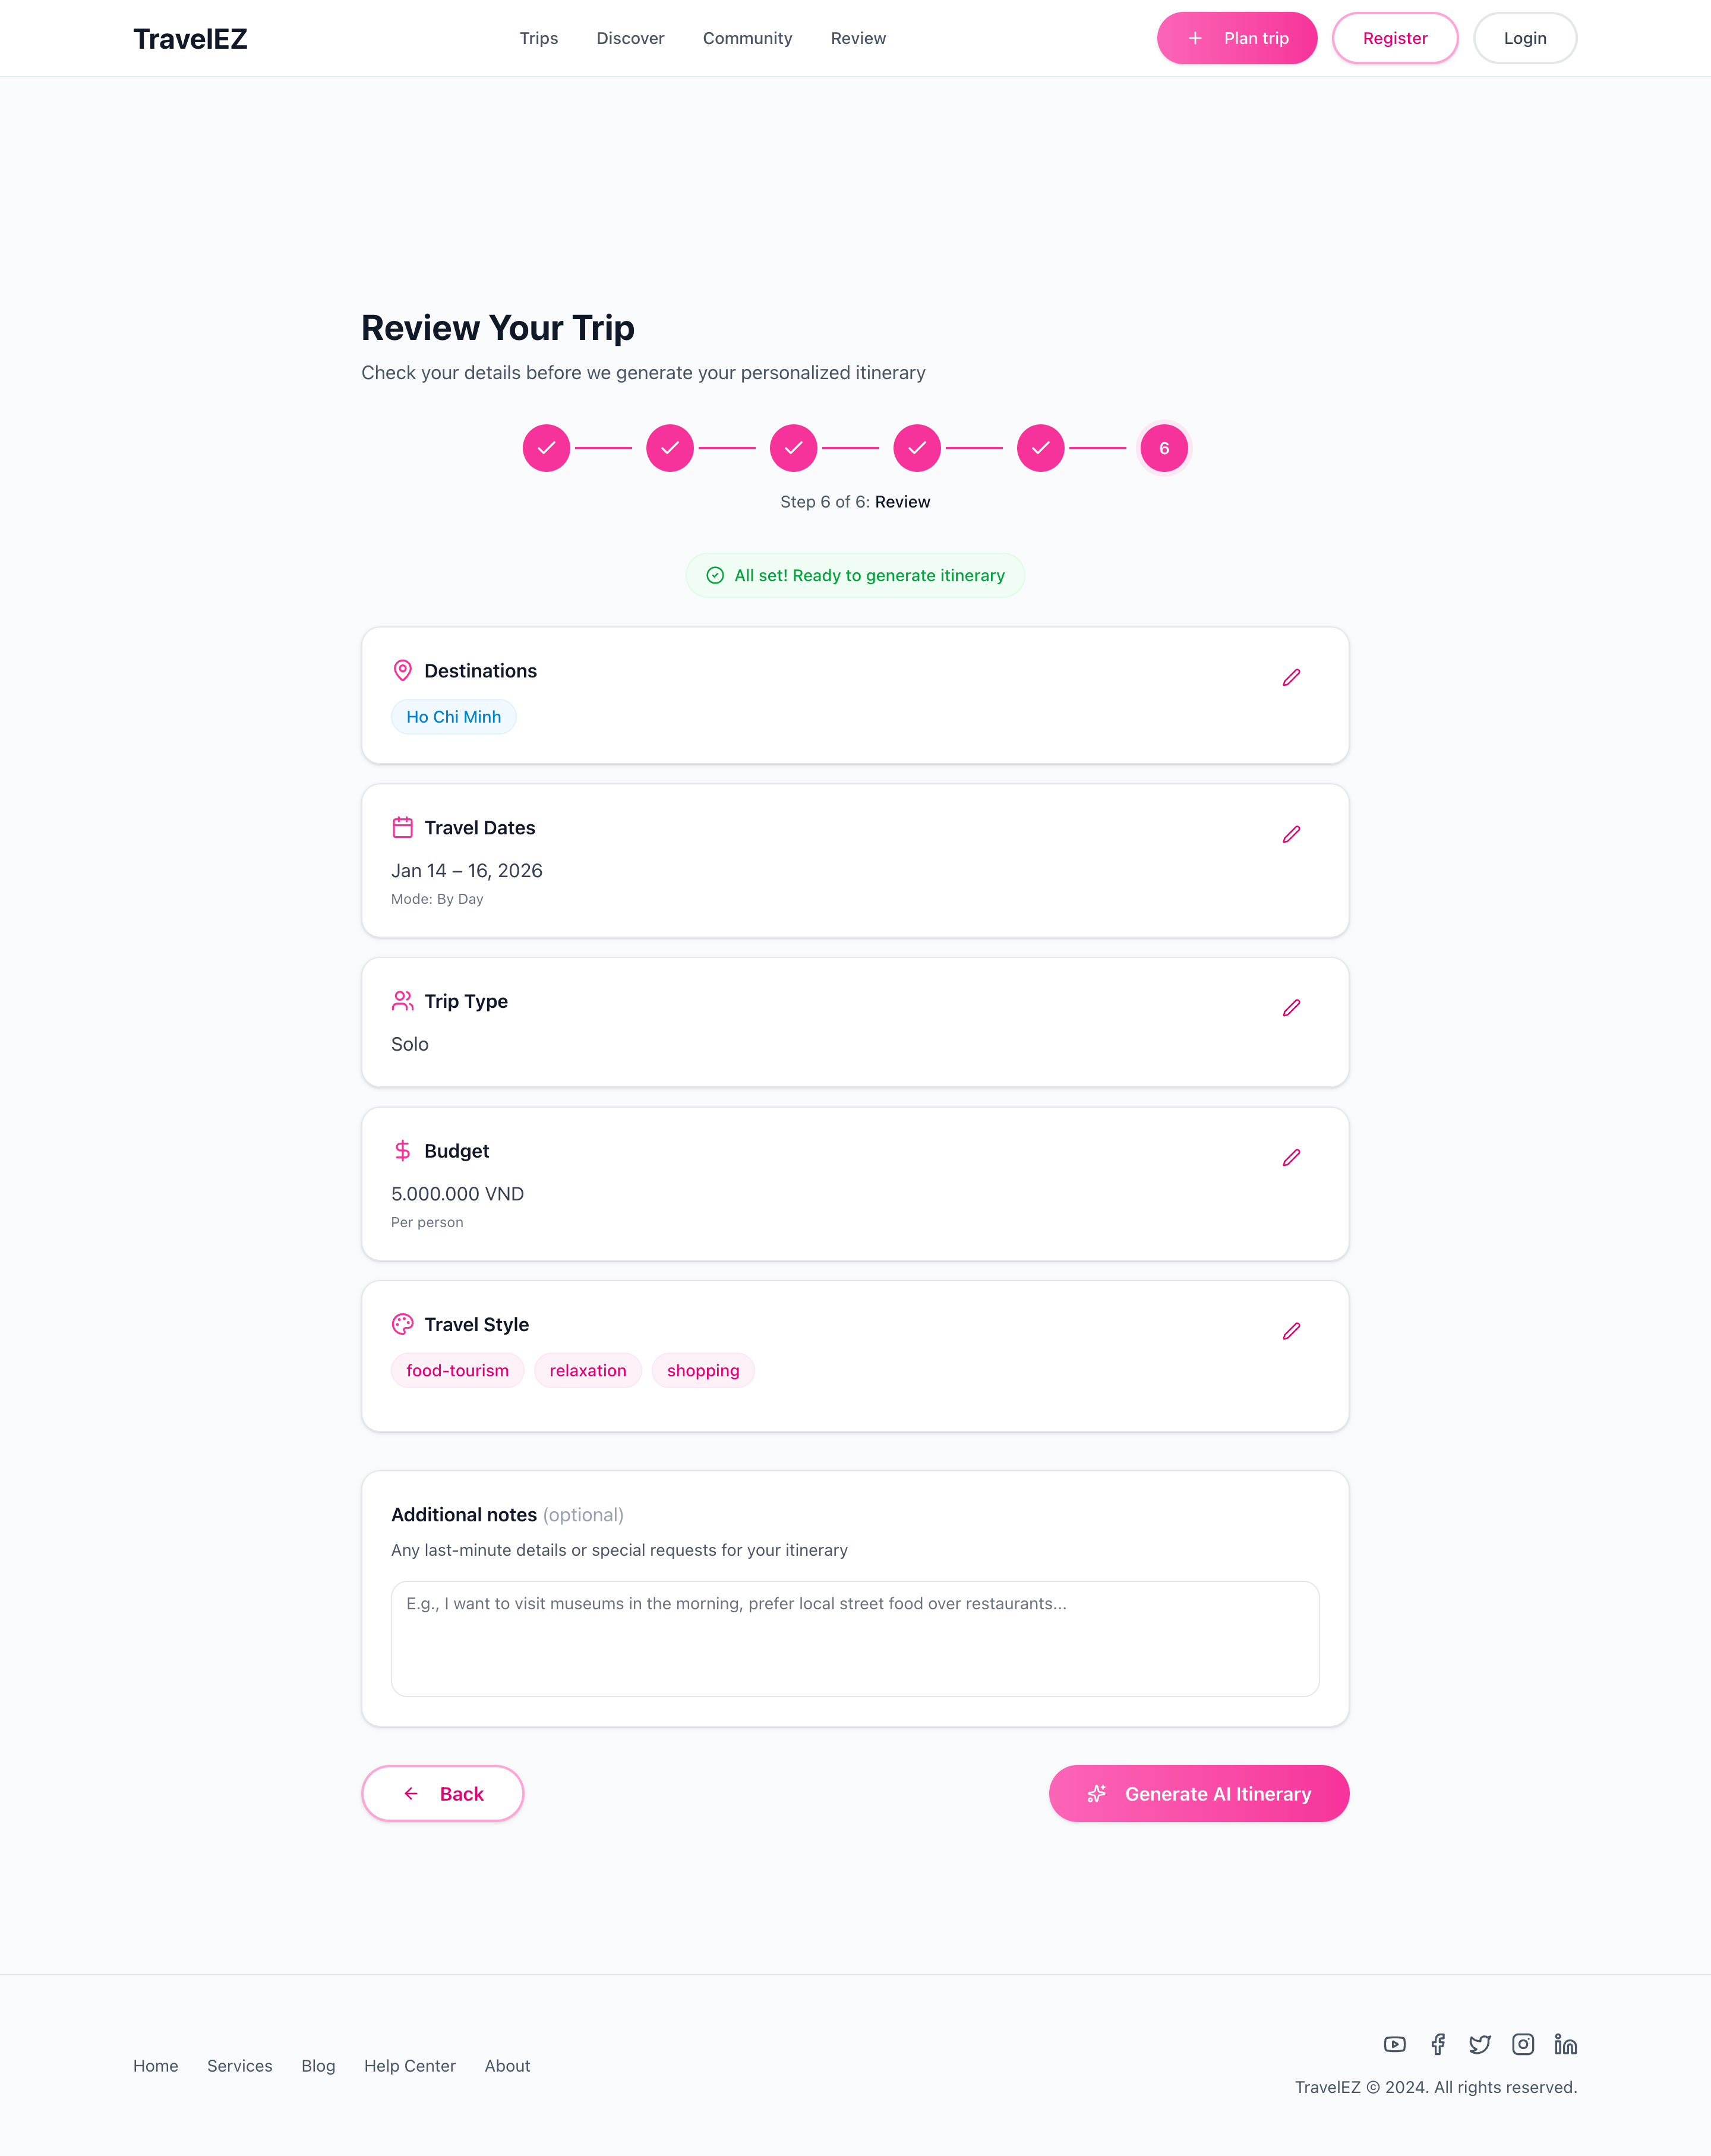
\includegraphics[width=1.0\linewidth]{Images/8. Implement/Itinerary-UI/localhost-3000-planning-summary.png}
    \caption{Giao diện Tổng quan: Xem lại và tạo lịch trình}
    \label{fig:summary}
    
    \vspace{0.5cm}
    \raggedright
    \textbf{Bước 6 - Tổng hợp và Kích hoạt AI:} Hiển thị toàn bộ thông tin để kiểm tra lần cuối. Nút "Generate AI Itinerary" sẽ gửi ngữ cảnh xuống Backend để sinh lộ trình.
\end{figure}